%%%%%%%%%%%%%%%%%%%%%%%%%%%%%%%%%%%%%%%%%%%%
%%% MIRACLE WORKING
%%%%%%%%%%%%%%%%%%%%%%%%%%%%%%%%%%%%%%%%%%%%


\mysection{Miracle Working}{marvels-miracle-working}

\example {

    Faith Dice are used to perform Miracles.  Miracles must be performed on Hallowed Ground (a shrine, church, etc.) dedicated to your Small God, and you must have a \mylink{Holy Symbol}{miracle-holy-relic} \\~
    \\~
    Each Faith Die spent is removed from your Pool (as if you had rolled a 1 or a 2).

}



\mysubsection{Ambrosia}{miracle-ambrosia}

You can create \DICE d4 \UD of Provisions. These \UD can be combined into a single \UD (see "Adding and Splitting Usage Dice" in the Arbiter's Miscellany section of the core rules). These Provisions can be stored for use later, but it also particularly nourishes the faithful.  During the working of the Miracle, up to \DICE disciples of the Small God can partake of the Ambrosia and gain +1 Faith Die (the miracle worker cannot gain this benefit). Disciples partaking of the meal do not affect the \UD produced in any way.

\cbreak

\mysubsection{Covenant}{miracle-covenant}

You seal a bargain between yourself (the Suzerain) and another (the Vassal) by awarding your Small God temporary control over your collective \myital{noumenon} (this means that the Unhallowed can't be held to a Covenant).  A Covenant has to be given freely, but can be compelled by other factors (like a dagger to the throat).

Spend a number of \DICE equal to or greater than the \LVL of the Vassal and gain the following effects:

\mybullet { 
  \item You can give and take Faith from the Vassal as if they were a disciple (see the Mystic Virtue "Fishers of Men" in the core rules).
  \item You always know where your Vassal is and feel any strong emotions (lust, hatred, etc) or  physical extremes ("he's somewhere very, very cold") they might be enduring
  \item You can't directly harm your Vassal (though you can command others to do so); your Vassal isn't likewise constrained
  \item Your Vassal is immediately converted to the worship of your Small God
  \item Your Vassal barely needs sleep, and eats and drinks sparingly (roll Provisions \UD twice and take the higher roll).
  \item Your Vassal is affected as if they were under the effects of \mylink{Tongues of Fire}{miracle-tongues-of-fire} at all times
  \item Your Vassal gains +\DICE points of "holy armor".  Damage is subtracted from this total first before it is applied to Armor, Grit, etc.  It can't be healed, but it can be restored during a Vacation by worshiping at a shrine, church, etc. dedicated to your Small God
}

You and your Vassal can only have a single Covenant at any time.  The Covenant can be broken by one of you having a Crisis of Faith; the death of you or your Vassal; or by mutual, peaceful agreement.

\newpage

\mysubsection{Crusade}{miracle-crusade}

Transforms your Vassal into a Paladin of the Faith.

  \begin{center}
  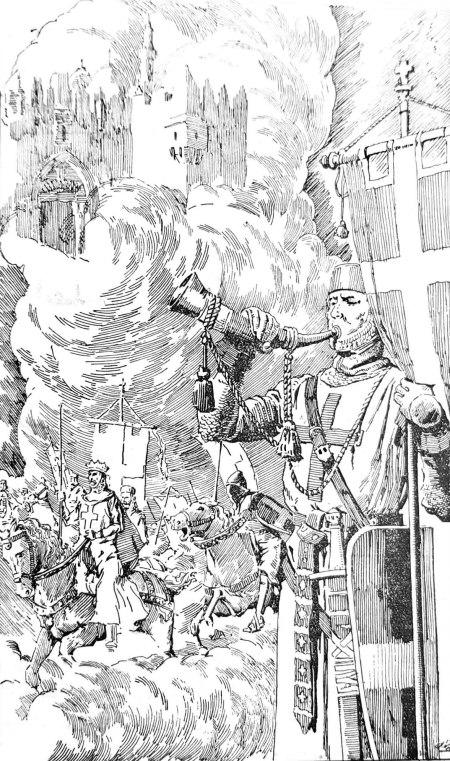
\includegraphics[scale=.5]{Crusade}
  \end{center}


Spend a number of \DICE equal to the \LVL x2 of the Vassal and gain the following effects (in addition to the benefits of being a Vassal):

\mybullet { 
  \item Your Vassal can use their Faith as if they were a Sellsword's Deed Die.  If they're already a Sellsword, they now have 2 Deed Dice they can roll together or separately.
  \item Your Vassal can gain Faith on their own (they don't need you to give it to them) up to a \MAX of 4 
  \item Your Vassal can cast any of the Seven Sacraments using their *Faith* Dice (see the Mystic Virtue "Gift of Grace" in the core rules)
}

You must name a \myital{jihad} important to your Small God: "wipe out the infidels of the Crawling Chaos", for example, or "bring the fingerbone of St. Sebastien to the reliquary in the Howling Wastes".  Similar to a Geas, any day not spent in the furtherance of the cause of the Crusade will lose your Vassal a single Faith die.  It's important to note that if your Vassal should lose all their Faith and suffer a Crisis of Faith, the Crusade has failed and the Covenant is broken.



\mysubsection{Golem}{miracle-golem}

A golem is a mortal-like figure, brought to life through magic.  Creating a golem requires gold for materials and effort in addition to spending Faith Dice:

\mytable{X c c} {
  \thead{Type} & \thead{\COST} & \thead{Faith Dice} \\
} {
  Paper  & 50\AU  & 8 \\
  Glass  & 100\AU  & 10 \\
  Wood  & 500\AU  & 12 \\
  Clay  & 1,000\AU  & 14 \\
}

Golems requires a \myital{shem} - a slip of paper with a magical rune written on it through the miracle of the \mylink{Holy Writ}{miracle-holy-writ}.

Golems are completely obedient to you and respectful of other followers of your Small God; presenting a Holy Symbol of your Small God is enough to keep them at bay, but only you can command them.  If you should die, the golem will continue performing your last command in perpetuity.

\mybold{Golems are immune to magic of any kind - including arcana and magical weapons.}

\myhighlight{Paper Golem}{miracle-paper-golem}

Paper golems are small (less than 100cm tall) creatures created for menial work.  They can carry a single Significant Item provided it doesn't weight more than 5kg (or a number of Insignificant Items up to 5kg).  Paper golems can "fly" on gusts of wind (similar to how a chicken can "fly") and walk and run as fast as a small child.  Paper golems record everything they see.  At any time, you can ask them a single question ("what was it you saw when you were in the Baron's chamber?", for example) and the golem will flatten itself into a scroll upon which is written what it "saw". The Golem remains a scroll forever more, with the symbol of the Small God embossed on the bottom of the scroll.  These embossed scrolls are very, very difficult to counterfeit - and the price if you get caught is high, as it would bring down the wrath of the entire church of your Small God.

Paper Golems are immune to non-magical fire, but immediately destroyed by magical flames.

\myhighlight{Glass Golem}{miracle-glass-golem}

Glass golems are 2m tall automatons filled with pungent herbs and combustibles called "smokes".  You determine the type of smoke at the point of creation. Glass golems immediately explode when dealt a forcible blow - a hit with a weapon, a fall from a height greater than 3m, etc.  The effect of exploding a Glass Golem deals d6 damage to everything Nearby (Save negates) as well as the following effects:

1. Smoke of Chaos:  every Nearby creature is Befuddled and Enraged (1-3 on a d6) or Afraid (4-6 on a d6)
2. Smoke of Heroes:  every Nearby Ally receives a 1 dice Blessing, and are immune to fear of any kind - but they can't retreat.
3. Smoke of the Holy: explodes to create Hallowed Ground in a circle 15m in radius; this can be used to create Hallowed Earth, or dispel Unhallowed Earth (if the radius is less than 15m).  Unhallowed creatures Close to the explosion are thrown 15m Nearby (treat as Falling Damage).
4. Smoke of Medicines: every Nearby Ally heals to \MAX Flesh and Grit

the smoke persists for Minutes, but can be dispersed by wind.  You are not limited to these options; they should discuss with the Arbiter if they wish to go a different way.


\myhighlight{Wood Golem}{miracle-wood-golem}

Wood golems are 3m docile, hulking, tree-like creatures possessing great strength. They are able to carry up to 50 Significant Items in their branches weighing up to 1,000kg total.  They can successfully break down non-magical doors, bend iron bars, and perform other feats of strength on a 4-in-6 (this number can be adjusted at the Arbiter's discretion).  They walk at a slow, shuffling gate (d3 \MD)

Wood golems will never attempt to defend themselves.  They can take up to 50 points of damage - Chopping weapons deal double-damage, and fire deals triple-damage.  They will mindlessly stand wherever you command: in front of a doorway, in the middle of a fire, or charging dumbly into a group of Monsters.

\myhighlight{Clay Golem}{miracle-clay-golem}

Clay golems are giant (4m tall) faceless creatures created to protect or guard an area.  You must tell them what they must guard at the moment of their creation, and they cannot stray further than 100m from that spot.  The spot they guard must be Hallowed, and if this ever ceases to be they will immediately crumble to dust.

Clay golems house the \myital{noumenon} of a Vassal or Paladin of their Maker (see \mylink{Covenant}{miracle-covenant} and \mylink{Crusade}{miracle-crusade}).  Your Vassal is ritually slain, and their blood is mixed with sacred earth and fire to create the clay giant. Your Vassal does not need to be a willing sacrifice, but remember you can't directly harm your Vassal.  The Clay Golem has all of the memories, skills, saves, and abilities of their Mortal form (including Deed Dice, spell casting,
etc.) and Grit, Flesh, etc.  They have a Soak: 2 and do 2d8 damage (2 Close).  They are immune to spells of the Mind paradigm, backstab, surprise, and Toxins. They cannot speak and are have unswerving obedience.

Clay golems can house the spirits of willing heroes (paladins who wish to protect the temple forever) or with those of unwilling enemies (forced to guard a forgotten hallway, or the temple of a heretic Small God).  When slain, the *noumenon* of the deceased do not travel to the Isle of the Dead.  None know what happens to their souls. 


\mysubsection{Hallowed Ground}{miracle-hallowed-ground}

You can either desecrate \mylink{Unhallowed Earth}{occultism-unhallowed-earth}, or create Hallowed Ground for performing miracles, somewhere within \DICE km of you.  You create / desecrate an area \DICE x \DICE meters in diameter.  If you're attempting to desecrate Unhallowed Earth, the diameter must be equal to or exceed the area of the Unhallowed Earth.  You must create a \mylink{Holy Write}{miracle-holy-writ} that will be consumed during the miracle; this Holy Writ identifies the Hallowed Ground as "belonging" to your Small God.  Another Mystic will know the size of the Hallowed Ground just by looking at it, but only other Mystics who worship your Small God will know which God the Hallowed Ground belongs to.


Hallowed Ground provides the following benefits:

\mylist {
  \item no Unseelie or Unhallowed creature may enter Hallowed Ground
  \item all Mortals inside the radius of the Hallowed Ground can immediately end a Markovian effect
  \item all Mystics on Hallowed Ground may ignore the negative effect of a Failure when using their Grace (that is, they may keep their Grace die even if they roll a 1 or a 2).
}

This miracle is the only one that does \mybold{not} require Hallowed Ground to perform.

\mysubsection{Holy Relic}{miracle-holy-relic}

A repository for Faith.  You can spend \DICE Faith and place them in the relic at the time of its creation.  This Faith can be used by other Mystics of your Small God (as well as yourself).  The relic itself must be something "special" - a fingerbone of a Saint, a shroud, etc.  - at the Arbiter's discretion.  The more powerful the relic, the more Faith can be placed inside of it.

The Miracle of the Holy Relic is used to create \mylink{Holy Symbols}{liturgies-holy-symbol}.  The symbol must be what is indicated under your Small God.  A Holy Symbol only requires you to spend a single Faith [die]

  \begin{center}
  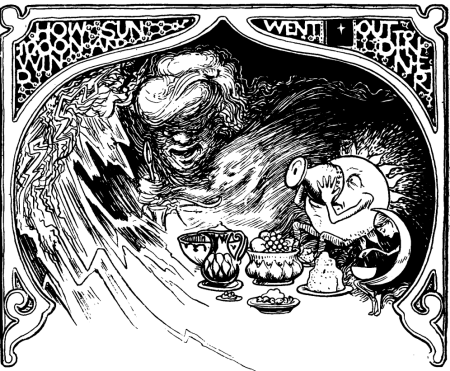
\includegraphics[scale=.5]{Miracle_1}
  \end{center}


\mysubsection{Holy Water}{miracle-holy-water}

You can spend \DICE Faith to create \DICE d4 \UD of Holy Water.  These \UD can be combined into a single \UD (see "Adding and Splitting Usage Dice" in the Arbiter's Miscellany section of the core rules). For each Faith Die spent, you must spend 25\AG in materials.

\mysubsection{Holy Writ}{miracle-holy-writ}

The word and the law of your Small God, written as seven sacred words known only to the faithful.  Only you and other members of your faith can see the words; to others, they look like random squiggles, strange designs, or "primitive" carvings.  Contained in the seven words is the Mystic who performed the Miracle, but you will need to make a successful Skill: Lore check to identify them unless you know them personally.   The Holy Writ only requires you to spend a single Faith [die]


\mysubsection{Incorruptibility}{miracle-incorruptibility}

This Miracle can be performed on a corpse to stop it from rotting.  The length of time depends on the number of Faith dice invested:  1 [die]: \SUMDICE Days; 3 \DICE: \SUMDICE Weeks; 5 \DICE: \SUMDICE Years; 7 \DICE: \SUMDICE Centuries; 9 \DICE: \SUMDICE Millennia.  So long as the body remains on Hallowed ground, it does not decay in any way and cannot be targeted with any spells from the Necromancy paradigm.  If the body is removed from Hallowed ground, it will begin to decay as normal.

\mysubsection{Proselytize}{miracle-proselytize}

You can attempt to convert others to the faith of your Small God, or give willing congregants instruction in the ways of your religion.  

You can spend 1 Faith die on as many Mortals (not Unseelie) as you choose, provided they are not Mystics who follow a different Small God.

The effects vary depending on whether the congregant is willing, apathetic, or unwilling

\mylist {

\item Willing:  you give one of your Faith Die to the worshiper
\item Apathetic:  roll the Faith \POOL; on a failure, the die is lost.  On success you have converted them - instead of giving your Faith Die to them, they gain one of their own
\item Unwilling:  the congregant gets a Save vs Doom.  If they succeed, you lose 2 Faith Die (the original you tried to give them, plus one other).  If they fail, roll as "Apathetic" above - if you succeed in converting them, you gain +1 Faith
}

Worshipers who have a Faith Die from you become your Disciple if you have the Mystic Virtue "Fishers of Men" (see core rules).

\mysubsection{Sacred Mass}{miracle-sacred-mass}

You can perform a sacred ceremony for \SUMDICE others (excluding yourself).  Non-Mystics who indulge in a Sacred Mass are Blessed for the remainder of the Session (or for the next Session at the Arbiter's discretion).  If you are a Mystic of a different Small God then the miracle worker and partake in the Mass, you lose 2 Faith Die.  If you are the miracle worker, or a Mystic of the same Small God, you gain 1 Faith Die for every 10 people participating up to your \MAX.



\mysubsection{Sin Eating}{miracle-sin-eating}

You can heal up to \DICE serious and non-serious Spirit Wounds on yourself or others

\cbreak

\mysubsection{Tongues of Fire}{miracle-tongues-of-fire}

Recipients of Tongues of Fire can speak (but not read) any Language they choose at will, and can command a single creature once per Session (see below).  The recipient can never lie while under the effects of Tongues of Flame.  Unwilling creatures get a Save.  This miracle lasts only for the Session (unless provided by Covenant). Up to \SUMDICE people other than you can be affected. 


\MYSTERY [
  Name= Command,
  Link=miracle-command,
  Paradigm=Mind,
  Save=Y,
  Duration=0 ,
  Counter= n/a  ,
  Keywords=None ,
  Target=Nearby creature
]

You shout a \DICE (1 in the case of Tongues of Fire) word command to the target, who must then carry it out if the fail a Save.  If the command would last more than a single Moment, the target gets a new Save at the beginning of each Moment.

